\documentclass{BeamerTemplate}

\title{Chapitre 3 -- Estimations et tests d'hypothèse (2\textsuperscript{e} partie)}
\subtitle{STT-1920 Méthodes statistiques}
\date{}

% Styles des graphiques
\pgfplotsset{
  base/.style={
    tick label style={font=\scriptsize}, label style={font=\small},
    title style={font=\small\bfseries},
    yticklabel style={/pgf/number format/fixed, /pgf/number format/precision=2},
    scaled y ticks=false,
  }
}

\begin{document}

\begin{frame}[t]
  \titlepage
\end{frame}

%===============================================================================
\section{Notion d'intervalle de confiance}
%===============================================================================

\begin{frame}[t]{Limite de l'estimation ponctuelle}
  Dans la première partie (chapitre 3a), nous avons vu que :
  \begin{itemize}\itemsep 2mm
    \item L'estimateur ponctuel $\overline{X}$ fournit \alert{une seule valeur} pour estimer le paramètre $\mu$.
    \item Parce que $\overline{X}$ est une variable aléatoire, sa valeur change d'un échantillon à l'autre.
    \item Pour l'exemple 1 de la pression ($n=7$), nous avons obtenu $\bar{x} = 134\text{ mm\,Hg}$.
  \end{itemize}

  \uncover<2->{
  \begin{Boite}{Une question fondamentale}
    Quelle confiance accorder à cette unique valeur 134? À quelle distance de la vraie moyenne inconnue $\mu$ a-t-on des chances de se trouver?
  \end{Boite}
  }

  \vspace{-2mm}
  \uncover<3->{
    $\Rightarrow$ On souhaite encadrer $\mu$ par un intervalle $[L_1, L_2]$ associé à un \alert{degré de certitude contrôlé}.
  }
\end{frame}

\begin{frame}[t]{Définition d'un intervalle de confiance}
  \begin{Boite}{Intervalle de confiance de niveau $1 - \alpha$}
    Deux statistiques $L_1$ et $L_2$ calculées à partir de l'échantillon telles que
    \vspace{-2mm}
    $$P(L_1 \le \theta \le L_2) = 1 - \alpha.$$
  \end{Boite}

  \vspace{-1mm}
  \begin{itemize}\itemsep 2mm
    \item<1-> $\theta$ est le \alert{paramètre inconnu} (valeur fixe de la population).
    \item<2-> $1 - \alpha$ est le \alert{niveau de confiance} (typiquement $90\%$, $95\%$ ou $99\%$).
    \item<3-> $\alpha$ est le \alert{seuil de risque} (probabilité que l'intervalle rate la vraie valeur).
    \item<4-> Lorsque l'intervalle est symétrique autour de l'estimation, on écrit
      $$\text{Estimation} \pm \text{Marge d'erreur}.$$
      \vspace{-4mm}

      La \alert{marge d'erreur} (ME) est la demi-longueur de l'intervalle.
  \end{itemize}
\end{frame}

\begin{frame}[t]{Que veut dire « confiance à 95\% »?}
  \begin{columns}[T]
    \column{0.52\textwidth}
      \centering
      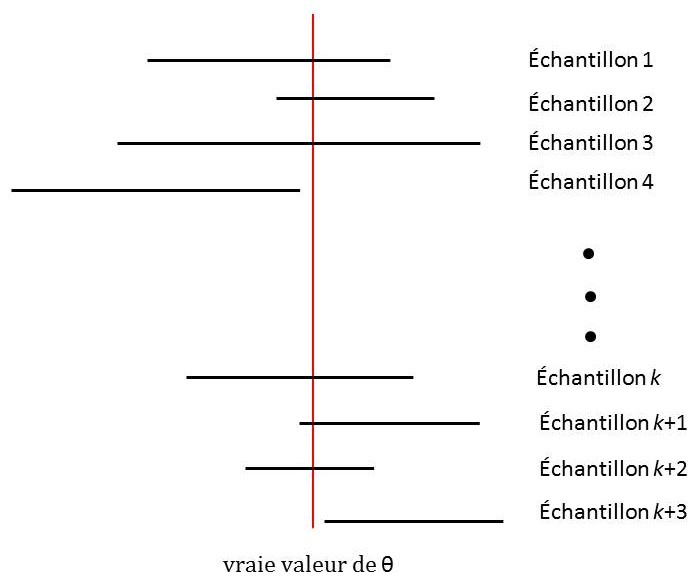
\includegraphics[width=\linewidth]{images/interpret-ic2.jpg}

    \column{0.45\textwidth}
      \small
      \begin{itemize}\itemsep 3mm
        \item Chaque échantillon donne un intervalle \alert{différent} (centre et longueur).
        \item La vraie valeur $\theta$ (ligne rouge) est \alert{fixe}.
        \item<2-> Certains intervalles la contiennent, d'autres la ratent (ex. : échantillons 4 et $k+3$).
        \item<3-> Le niveau de confiance est la proportion des intervalles qui contiennent $\theta$ \alert{à long terme}.
      \end{itemize}
  \end{columns}
\end{frame}

\begin{frame}[t]{Simulation : 40 intervalles de confiance à 90\%}
  \small
  40 échantillons de taille $n=7$ tirés d'une population $\mathcal{N}(\mu = 133,\ \sigma^2 = 62)$ (comme au chapitre 3a).
  Pour chacun, on calcule l'IC à 90\% pour $\mu$ (formule vue plus loin).

  \centering
  \begin{tikzpicture}
    \begin{axis}[
      base, width=0.95\textwidth, height=5.3cm,
      xmin=0, xmax=41, ymin=119, ymax=149,
      xlabel={Échantillon}, ylabel={Pression (mm\,Hg)},
      xtick={1,5,10,15,20,25,30,35,40},
      label style={font=\scriptsize},
    ]
      \draw[rougelaval, thick] (axis cs:0,133) -- (axis cs:41,133);
      \node[rougelaval, font=\scriptsize, anchor=west, fill=Fond, inner sep=1pt] at (axis cs:0.3,146.5) {Ligne rouge : $\mu = 133$};
      \draw[black!70, line width=1pt] (axis cs:1,128.20) -- (axis cs:1,138.65);
      \draw[black!70, line width=1pt] (axis cs:2,126.37) -- (axis cs:2,140.20);
      \draw[Accent, line width=1.6pt] (axis cs:3,135.26) -- (axis cs:3,140.45);
      \draw[black!70, line width=1pt] (axis cs:4,124.41) -- (axis cs:4,136.73);
      \draw[black!70, line width=1pt] (axis cs:5,128.15) -- (axis cs:5,138.13);
      \draw[black!70, line width=1pt] (axis cs:6,130.38) -- (axis cs:6,137.34);
      \draw[black!70, line width=1pt] (axis cs:7,130.27) -- (axis cs:7,137.44);
      \draw[black!70, line width=1pt] (axis cs:8,130.33) -- (axis cs:8,143.10);
      \draw[black!70, line width=1pt] (axis cs:9,129.00) -- (axis cs:9,141.57);
      \draw[black!70, line width=1pt] (axis cs:10,126.93) -- (axis cs:10,142.21);
      \draw[black!70, line width=1pt] (axis cs:11,126.54) -- (axis cs:11,135.17);
      \draw[black!70, line width=1pt] (axis cs:12,126.57) -- (axis cs:12,136.00);
      \draw[black!70, line width=1pt] (axis cs:13,132.16) -- (axis cs:13,138.12);
      \draw[black!70, line width=1pt] (axis cs:14,130.68) -- (axis cs:14,142.75);
      \draw[Accent, line width=1.6pt] (axis cs:15,125.91) -- (axis cs:15,131.52);
      \draw[black!70, line width=1pt] (axis cs:16,132.37) -- (axis cs:16,143.34);
      \draw[black!70, line width=1pt] (axis cs:17,128.89) -- (axis cs:17,137.11);
      \draw[black!70, line width=1pt] (axis cs:18,130.22) -- (axis cs:18,138.06);
      \draw[black!70, line width=1pt] (axis cs:19,129.22) -- (axis cs:19,133.93);
      \draw[Accent, line width=1.6pt] (axis cs:20,124.25) -- (axis cs:20,132.32);
      \draw[black!70, line width=1pt] (axis cs:21,121.40) -- (axis cs:21,138.31);
      \draw[black!70, line width=1pt] (axis cs:22,124.38) -- (axis cs:22,133.33);
      \draw[black!70, line width=1pt] (axis cs:23,124.00) -- (axis cs:23,139.14);
      \draw[black!70, line width=1pt] (axis cs:24,127.78) -- (axis cs:24,141.65);
      \draw[black!70, line width=1pt] (axis cs:25,130.67) -- (axis cs:25,141.04);
      \draw[black!70, line width=1pt] (axis cs:26,132.33) -- (axis cs:26,144.53);
      \draw[black!70, line width=1pt] (axis cs:27,126.81) -- (axis cs:27,138.05);
      \draw[black!70, line width=1pt] (axis cs:28,125.22) -- (axis cs:28,134.49);
      \draw[black!70, line width=1pt] (axis cs:29,131.52) -- (axis cs:29,143.33);
      \draw[black!70, line width=1pt] (axis cs:30,126.40) -- (axis cs:30,143.03);
      \draw[black!70, line width=1pt] (axis cs:31,128.27) -- (axis cs:31,139.44);
      \draw[black!70, line width=1pt] (axis cs:32,124.39) -- (axis cs:32,133.89);
      \draw[black!70, line width=1pt] (axis cs:33,124.19) -- (axis cs:33,137.53);
      \draw[black!70, line width=1pt] (axis cs:34,121.75) -- (axis cs:34,135.68);
      \draw[black!70, line width=1pt] (axis cs:35,132.50) -- (axis cs:35,141.21);
      \draw[black!70, line width=1pt] (axis cs:36,125.95) -- (axis cs:36,136.91);
      \draw[black!70, line width=1pt] (axis cs:37,126.26) -- (axis cs:37,139.74);
      \draw[black!70, line width=1pt] (axis cs:38,131.39) -- (axis cs:38,140.89);
      \draw[Accent, line width=1.6pt] (axis cs:39,126.03) -- (axis cs:39,131.97);
      \draw[black!70, line width=1pt] (axis cs:40,125.83) -- (axis cs:40,144.75);
    \end{axis}
  \end{tikzpicture}

  \raggedright
  \uncover<2->{\alert{36 intervalles sur 40 (90\%)} contiennent $\mu$ ; les 4 intervalles orange la ratent.}
\end{frame}

\begin{frame}[t]{Interprétation rigoureuse}
  \begin{Boite}{\faCheckCircle\ Interprétation correcte}
    \small
    Si on prélevait un grand nombre d'échantillons de même taille $n$ et que pour chacun on construisait l'intervalle à 95\%, alors \alert{environ 95\% de ces intervalles contiendraient la vraie valeur $\theta$}.
  \end{Boite}

  \vspace{-3mm}
  \uncover<2->{
  \begin{Boite}{\faTimesCircle\ Attention aux interprétations incorrectes !}
    \small
    \begin{itemize}\itemsep 1mm
      \item \textbf{Faux :} « Il y a 90\% de chances que $\mu$ appartienne à $[129{,}39 \,;\, 138{,}61]$. »
        $\rightarrow$ $\mu$ n'est pas aléatoire : c'est l'intervalle $[L_1, L_2]$ qui l'est !
      \item \textbf{Faux :} « 90\% des individus ont une valeur entre $129{,}39$ et $138{,}61$. »
        $\rightarrow$ L'IC vise la \emph{moyenne} $\mu$, pas les individus !
    \end{itemize}
  \end{Boite}
  }
\end{frame}

\begin{frame}[plain,t]
  \centerline{\LARGE\bfseries\alert{QUIZ !}}

  \medskip
  Dans la simulation précédente (40 intervalles à 90\%) :
  \begin{itemize}\itemsep 1.2cm
    \item Combien d'intervalles s'attendait-on à voir rater $\mu$?
    \item<2-> Si on avait plutôt calculé des IC à 95\%, combien en moyenne rateraient $\mu$? Les intervalles seraient-ils plus longs ou plus courts?
    \item<3-> Pourquoi les 40 intervalles n'ont-ils pas tous la même longueur?
  \end{itemize}
\end{frame}

%===============================================================================
\section{Construction de l'intervalle pour la moyenne}
%===============================================================================

\begin{frame}[t]{Cas théorique : si $\sigma$ était connue}
  Supposons $X_1, \ldots, X_n$ i.i.d. de loi $\mathcal{N}(\mu, \sigma^2)$, avec $\sigma$ \alert{connue}.
  $$\overline{X} \sim \mathcal{N}\left(\mu,\, \frac{\sigma^2}{n}\right) \quad \Longrightarrow \quad Z = \frac{\overline{X} - \mu}{\sigma/\sqrt{n}} \sim \mathcal{N}(0, 1)$$

  \vspace{-2mm}
  \uncover<2->{
  Pour un niveau $1 - \alpha$, on prend le quantile $z_{\alpha/2}$ tel que $P(Z > z_{\alpha/2}) = \alpha/2$ :
  $$P\left(-z_{\alpha/2} \le \frac{\overline{X} - \mu}{\sigma/\sqrt{n}} \le z_{\alpha/2}\right) = 1 - \alpha$$
  }

  \vspace{-4mm}
  \uncover<3->{
  \begin{Boite}{IC pour $\mu$ ($\sigma$ connue) en isolant $\mu$ au centre}
    $$\left[ \overline{X} - z_{\alpha/2}\,\frac{\sigma}{\sqrt{n}}, \; \overline{X} + z_{\alpha/2}\,\frac{\sigma}{\sqrt{n}} \right]
    \qquad {\small(z_{0{,}05} = 1{,}645,\ z_{0{,}025} = 1{,}96,\ z_{0{,}005} = 2{,}576)}$$
  \end{Boite}
  }

  \vspace{-2mm}
  \uncover<4->{
    \alert{Le problème pratique :} en réalité, on ne connaît presque jamais $\sigma$ !
  }
\end{frame}

\begin{frame}[t]{Que faire quand $\sigma$ est inconnue?}
  Puisque $\sigma$ est inconnue, l'idée naturelle est de la remplacer par l'écart-type échantillonnal $S$ :
  $$T = \frac{\overline{X} - \mu}{S / \sqrt{n}}$$

  \vspace{-2mm}
  \begin{itemize}\itemsep 2mm
    \item<2-> Au dénominateur, $S$ n'est plus une constante, mais une \alert{variable aléatoire}.
    \item<3-> Cette incertitude supplémentaire rend $T$ \alert{plus dispersée} que la loi normale centrée réduite $Z$.
    \item<4-> $T$ ne suit plus une loi normale $\mathcal{N}(0,1)$ !
  \end{itemize}

  \uncover<5->{
  \begin{Boite}{Quelle est la loi exacte de $T$?}
    La réponse a été découverte en 1908 par William Sealy Gosset : la \alert{loi de Student}.
  \end{Boite}
  }
\end{frame}

\begin{frame}[t]{William Sealy Gosset (1876--1937)}
  \begin{columns}[T]
    \column{0.68\textwidth}
      \begin{itemize}\itemsep 3mm
        \item Chimiste et statisticien en chef à la brasserie \alert{Guinness} à Dublin.
        \item Travaillait avec de \textbf{très petits échantillons} (variétés d'orge, température de brassage, levures).
        \item Découvre la distribution exacte de $\frac{\overline{X}-\mu}{S/\sqrt{n}}$.
        \item Guinness interdisait à ses employés de publier des secrets d'entreprise : il publia en 1908 sous le pseudonyme \alert{« Student »}.
      \end{itemize}

    \column{0.28\textwidth}
      \centering
      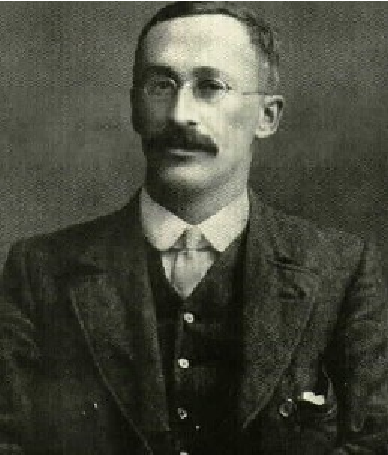
\includegraphics[width=\linewidth]{images/Gosset_1.pdf}

      {\tiny William Sealy Gosset}
  \end{columns}
\end{frame}

\begin{frame}[t]{La loi de Student $t_k$}
  \begin{Boite}{Théorème de Student}
    Si $X_1, \ldots, X_n \overset{iid}{\sim} \mathcal{N}(\mu, \sigma^2)$, alors
    $$T = \frac{\overline{X} - \mu}{S / \sqrt{n}} \sim t_{n-1},$$
    une \alert{loi de Student à $k = n - 1$ degrés de liberté}.
  \end{Boite}

  \vspace{-2mm}
  \begin{itemize}\itemsep 2mm
    \item<2-> Symétrique en 0, en forme de cloche, tout comme la loi normale.
    \item<3-> Ses \alert{queues sont plus lourdes} : les valeurs extrêmes sont plus probables en raison de la variabilité de $S$.
    \item<4-> Quand $k \to \infty$, la loi de Student \alert{converge vers la loi normale $\mathcal{N}(0,1)$}.
  \end{itemize}
\end{frame}

\begin{frame}[t]{Comparaison de la loi normale et des lois de Student}
  \begin{center}
  \begin{tikzpicture}
    \begin{axis}[
      base, width=10.5cm, height=5.5cm,
      xmin=-4, xmax=4, ymin=0, ymax=0.45,
      xlabel={$t$}, ylabel={Densité},
      legend pos=north east, legend style={font=\scriptsize}
    ]
      % Normale N(0,1)
      \addplot[thick, black, domain=-4:4, samples=100]
        {exp(-x^2/2) / sqrt(2*pi)};
      \addlegendentry{$\mathcal{N}(0,1)$}

      % Student k=2: f(x) = 1 / (2 * (1 + x^2/2)^(3/2))
      \addplot[thick, rougelaval, dashed, domain=-4:4, samples=100]
        {1 / (2*sqrt(2) * (1 + x^2/2)^1.5)};
      \addlegendentry{Student $k = 2$}

      % Student k=10
      \addplot[thick, Dominante, domain=-4:4, samples=100]
        {0.3891 / ((1 + x^2/10)^5.5)};
      \addlegendentry{Student $k = 10$}
    \end{axis}
  \end{tikzpicture}
  \end{center}

  \vspace{-2mm}
  Pour $k$ petit, les quantiles sont plus grands que $1{,}96$ pour compenser l'incertitude sur $\sigma$
  (ex. : $t_{6,\,0{,}025} = 2{,}447$ ; $t_{29,\,0{,}025} = 2{,}045$).
\end{frame}

\begin{frame}[t]{Formule de l'IC pour $\mu$ ($\sigma$ inconnue)}
  \begin{Boite}{Intervalle de confiance pour la moyenne $\mu$}
    Soit un échantillon aléatoire d'une population normale :
    $$\left[ \overline{X} - t_{n-1,\, \alpha/2} \, \frac{S}{\sqrt{n}}, \; \overline{X} + t_{n-1,\, \alpha/2} \, \frac{S}{\sqrt{n}} \right]$$
  \end{Boite}

  \vspace{-1mm}
  \uncover<2->{
  \begin{itemize}\itemsep 2mm
    \item $\overline{X}$ : estimation ponctuelle de la moyenne.
    \item $\frac{S}{\sqrt{n}}$ : erreur-type estimée ($\widehat{\text{ET}}$).
    \item $t_{n-1,\, \alpha/2}$ : valeur critique de la table de Student à $n-1$ d.l.\\ (dans R : \texttt{qt(1-alpha/2, n-1)}).
    \item $\text{ME} = t_{n-1,\, \alpha/2} \, \frac{S}{\sqrt{n}}$ : la \alert{marge d'erreur}.
  \end{itemize}
  }
\end{frame}

\begin{frame}[t]{Exemple 1 (suite) : pression artérielle}
  Mesures ($n=7$) : 141, 130, 135, 138, 137, 122, 135 ; \ $\bar{x} = 134\text{ mm\,Hg}$, \ $s = 6{,}27\text{ mm\,Hg}$.

  On cherche un intervalle de confiance à \alert{$90\%$}, donc $\alpha = 0{,}10$ et $\alpha/2 = 0{,}05$.

  \medskip
  \uncover<2->{
  \begin{enumerate}\itemsep 2mm
    \item \textbf{Degrés de liberté :} $k = n - 1 = 7 - 1 = 6$.
    \item \textbf{Quantile critique :} dans la table de Student, $t_{6,\, 0{,}05} = \mathbf{1{,}943}$.
    \item \textbf{Erreur-type estimée :} $\frac{s}{\sqrt{n}} = \frac{6{,}27}{\sqrt{7}} = \mathbf{2{,}37}$.
    \item \textbf{Marge d'erreur :} $\text{ME} = 1{,}943 \times 2{,}37 = \mathbf{4{,}61\text{ mm\,Hg}}$.
    \item \textbf{Intervalle de confiance à 90\% :}
      $[134 - 4{,}61 \,;\, 134 + 4{,}61] = \mathbf{[129{,}39 \,;\, 138{,}61]\text{ mm\,Hg}}$
  \end{enumerate}
  }

  \medskip
  \uncover<3->{
  \small Remarque : on garde toutes les décimales dans les calculs intermédiaires ($s/\sqrt{n} = 2{,}3705$), puis on arrondit à la fin.
  }
\end{frame}

\begin{frame}[fragile,t]{Avec R}
  \small
\begin{verbatim}
> x <- c(141, 130, 135, 138, 137, 122, 135)
> t.test(x, conf.level = 0.90)$conf.int
[1] 129.3938 138.6062
attr(,"conf.level")
[1] 0.9
> t.test(x)$conf.int          # niveau 95 % par défaut
[1] 128.1997 139.8003
\end{verbatim}

  \normalsize
  \begin{itemize}\itemsep 2mm
    \item La fonction \texttt{t.test()} affiche aussi un \alert{test d'hypothèses} ($t$, \texttt{p-value}) : nous verrons au chapitre 3c comment l'interpréter.
    \item Quantile à la main : \texttt{qt(0.95, df = 6)} donne $1{,}943$.
  \end{itemize}
\end{frame}

%===============================================================================
\section{Quiz conceptuel : Vrai ou Faux ?}
%===============================================================================

\begin{frame}[t]{Question 1}
  \begin{Boite}{Énoncé 1}
    « 90\% des gens de cette population ont une pression artérielle comprise entre $129{,}39$ et $138{,}61\text{ mm\,Hg}$. »
  \end{Boite}

  \bigskip
  \uncover<2->{
  \alert{\Large FAUX !}

  \medskip
  L'intervalle de confiance est construit pour estimer le paramètre moyen $\mu$ de la population, et non pas pour contenir 90\% des observations individuelles.
  La variabilité des individus est régie par $\sigma$ (environ $6{,}3$), alors que l'intervalle est basé sur $\sigma/\sqrt{n}$ (environ $2{,}4$).
  }
\end{frame}

\begin{frame}[t]{Question 2}
  \begin{Boite}{Énoncé 2}
    « 90\% des gens de cet échantillon ont une pression artérielle comprise entre $129{,}39$ et $138{,}61\text{ mm\,Hg}$. »
  \end{Boite}

  \bigskip
  \uncover<2->{
  \alert{\Large FAUX !}

  \medskip
  Pour le vérifier, regardons notre échantillon : $\{141, 130, 135, 138, 137, 122, 135\}$.
  \begin{itemize}
    \item 122 et 141 sont à l'extérieur de l'intervalle.
    \item Seules 5 des 7 valeurs ($71{,}4\%$) sont à l'intérieur !
  \end{itemize}
  L'intervalle ne prétend absolument pas décrire l'échantillon, il vise la \textbf{vraie moyenne $\mu$}.
  }
\end{frame}

\begin{frame}[t]{Question 3}
  \begin{Boite}{Énoncé 3}
    « Si on prenait des mesures sur 7 autres individus, il y a 90\% de chances que la moyenne $\overline{x}_{\text{nouveau}}$ de ce nouvel échantillon soit comprise entre $129{,}39$ et $138{,}61$. »
  \end{Boite}

  \bigskip
  \uncover<2->{
  \alert{\Large FAUX !}

  \medskip
  Une nouvelle moyenne $\overline{X}_{\text{nouv}}$ a sa propre variabilité autour de $\mu$.
  L'écart entre deux moyennes indépendantes a pour écart-type $\sqrt{\frac{\sigma^2}{n} + \frac{\sigma^2}{n}} = \sqrt{2}\,\frac{\sigma}{\sqrt{n}}$, qui est plus grand que $\frac{\sigma}{\sqrt{n}}$.
  Pour prédire une nouvelle moyenne ou observation, on utilise un \alert{intervalle de prédiction}.
  }
\end{frame}

\begin{frame}[t]{Question 4}
  \begin{Boite}{Énoncé 4}
    « Si on tirait 1000 échantillons de taille 7 dans cette population et qu'on calculait pour chacun l'IC à 90\%, environ 900 d'entre eux contiendraient la vraie moyenne $\mu$. »
  \end{Boite}

  \bigskip
  \uncover<2->{
  \textbf{\color{green!60!black}\Large VRAI !}

  \medskip
  C'est \alert{exactement} la signification probabiliste du niveau de confiance de 90\% (voir la simulation de 40 intervalles) !
  C'est le mécanisme de construction de l'intervalle qui est fiable à 90\%.
  }
\end{frame}

\begin{frame}[t]{Question 5}
  \begin{Boite}{Énoncé 5}
    « Avec un échantillon de taille $n \ge 30$, on peut utiliser les quantiles de la loi normale au lieu de la loi de Student. »
  \end{Boite}

  \uncover<2->{
  \textbf{\color{green!60!black}\Large VRAI (en pratique) !}

  \smallskip
  \begin{itemize}\itemsep 1mm
    \item Par le théorème limite central (TLC), la loi de $\overline{X}$ est approximativement normale même si la population ne l'est pas.
    \item De plus, pour $n \ge 30$, la loi de Student est presque identique à la normale : $t_{29,\, 0{,}025} = 2{,}045 \approx 1{,}96$.
    \item Avec un logiciel comme R, on utilise toutefois toujours la loi de Student.
  \end{itemize}
  }
\end{frame}

\begin{frame}[t]{Questions 6 et 7}
  \begin{Boite}{Énoncé 6}
    « Avec un échantillon plus grand, on obtiendrait un intervalle de confiance plus long. »
  \end{Boite}
  \vspace{-2mm}
  \uncover<2->{
    \alert{\textbf{FAUX :}} la longueur vaut $2\, t_{n-1,\,\alpha/2}\, \frac{s}{\sqrt{n}}$. Puisque $\sqrt{n}$ est au dénominateur, \textbf{plus $n$ augmente, plus l'intervalle est étroit}.
  }

  \uncover<3->{
  \begin{Boite}{Énoncé 7}
    « Si la vraie moyenne est de 133, l'estimation obtenue $\bar{x} = 134$ est biaisée. »
  \end{Boite}
  }
  \vspace{-2mm}
  \uncover<4->{
    \alert{\textbf{FAUX :}} le biais est une propriété de l'\emph{estimateur} ($E[\overline{X}] = \mu$). Une réalisation $\bar{x}$ n'est jamais exactement égale à $\mu$ en raison de l'aléa, sans que l'estimateur soit biaisé pour autant.
  }
\end{frame}

%===============================================================================
\section{Cas \texorpdfstring{$n$}{n} grand, marge d'erreur et taille d'échantillon}
%===============================================================================

\begin{frame}[t]{Et si la population n'est pas normale?}
  Plusieurs variables biologiques sont \alert{asymétriques} (concentrations de contaminants, charges parasitaires\ldots), alors que la formule de Student suppose la normalité.

  \uncover<2->{
  \begin{Boite}{{IC pour $\mu$ : loi inconnue, $n$ grand (en pratique $n \ge 30$)}}
    Par le TLC (chapitre 2), $\overline{X} \approx \mathcal{N}(\mu, \sigma^2/n)$ et $S \approx \sigma$. Un IC de niveau \alert{approximativement} $1-\alpha$ est
    \vspace{-1mm}
    $$\left[\overline{X} - z_{\alpha/2}\,\frac{S}{\sqrt{n}}, \; \overline{X} + z_{\alpha/2}\,\frac{S}{\sqrt{n}}\right].$$
    \vspace{-5mm}
  \end{Boite}
  }

  \vspace{-2mm}
  \uncover<3->{
  \small
  \begin{itemize}\itemsep 0mm
    \item Si $\sigma$ est connue, on l'utilise au lieu de $S$. Plus la population est asymétrique, plus $n$ doit être grand.
    \item $n$ petit et population très asymétrique : aucune formule fiable !
  \end{itemize}
  }
\end{frame}

\begin{frame}[t]{Exemple 3 : mercure dans la chair des dorés}
  On mesure la concentration de mercure ($\mu$g/g) dans la chair de $n = 50$ dorés jaunes pêchés dans un réservoir. La distribution est asymétrique à droite.
  On obtient $\bar{x} = 0{,}42\ \mu$g/g et $s = 0{,}18\ \mu$g/g.

  \medskip
  \textbf{Question :} donnez un IC à 95\% pour la concentration moyenne $\mu$.

  \medskip
  \uncover<2->{
  \begin{enumerate}\itemsep 2mm
    \item $n = 50$ est grand : on utilise le TLC et $z_{0{,}025} = 1{,}96$.
    \item Erreur-type estimée : $s/\sqrt{n} = 0{,}18/\sqrt{50} = 0{,}0255$.
    \item Marge d'erreur : $\text{ME} = 1{,}96 \times 0{,}0255 = 0{,}050\ \mu$g/g.
    \item IC à 95\% : $0{,}42 \pm 0{,}050 = \mathbf{[0{,}370 \,;\, 0{,}470]}\ \mu\text{g/g}$.
  \end{enumerate}
  }

  \medskip
  \uncover<3->{
    La ligne directrice de Santé Canada pour le poisson est de $0{,}5\ \mu$g/g : l'intervalle entier est sous cette valeur. Nous verrons au chapitre 3c comment formaliser cette conclusion par un \alert{test}.
  }
\end{frame}

\begin{frame}[t]{Marge d'erreur et erreur-type : une structure commune}
  Les trois intervalles pour $\mu$ ont la même forme :
  \begin{Boite}{Forme générale}
    \centering
    $\text{Estimation} \;\pm\; \underbrace{\text{quantile} \times \text{erreur-type}}_{\text{marge d'erreur}}$
    \qquad Longueur $= 2 \times \text{ME}$
  \end{Boite}

  \vspace{-3mm}
  \centering
  \small
  \renewcommand{\arraystretch}{1.2}
  \begin{tabular}{llll}\toprule
    \textbf{Situation} & \textbf{Estimation} & \textbf{Quantile} & \textbf{Erreur-type} \\ \midrule
    Normale, $\sigma$ connue & $\bar{x}$ & $z_{\alpha/2}$ & $\sigma/\sqrt{n}$ \\
    Normale, $\sigma$ inconnue & $\bar{x}$ & $t_{n-1,\,\alpha/2}$ & $s/\sqrt{n}$ \\
    Loi inconnue, $n$ grand & $\bar{x}$ & $z_{\alpha/2}$ & $s/\sqrt{n}$ \\ \bottomrule
  \end{tabular}

  \raggedright
  \smallskip
  \uncover<2->{
    Trois facteurs déterminent la marge d'erreur : la \alert{variabilité} ($\sigma$), la \alert{taille d'échantillon} ($n$) et le \alert{niveau de confiance} (quantile).
  }
\end{frame}

\begin{frame}[t]{Effet du niveau de confiance et de la taille d'échantillon}
  \small
  Exemple 1 : $\bar{x} = 134$, $s = 6{,}27$ (on suppose les mêmes $\bar{x}$ et $s$ pour les $n$ plus grands).

  \centering
  \begin{tikzpicture}
    \begin{axis}[
      base, width=0.92\textwidth, height=5.2cm,
      xmin=123, xmax=148, ymin=0.3, ymax=5.7,
      xlabel={Pression (mm\,Hg)},
      ytick={1,2,3,4,5},
      yticklabels={{$n=112$, 95\%}, {$n=28$, 95\%}, {$n=7$, 99\%}, {$n=7$, 95\%}, {$n=7$, 90\%}},
      yticklabel style={font=\scriptsize},
    ]
      \draw[gray, dashed] (axis cs:134,0.3) -- (axis cs:134,5.7);
      \draw[Dominante, line width=3pt] (axis cs:129.39,5) -- (axis cs:138.61,5);
      \draw[Dominante!70!black, line width=3pt] (axis cs:128.20,4) -- (axis cs:139.80,4);
      \draw[TitreBoite, line width=3pt] (axis cs:125.21,3) -- (axis cs:142.79,3);
      \draw[Accent, line width=3pt] (axis cs:131.57,2) -- (axis cs:136.43,2);
      \draw[Accent!70!black, line width=3pt] (axis cs:132.83,1) -- (axis cs:135.17,1);
      \node[font=\scriptsize, right] at (axis cs:138.9,5) {ME $= 4{,}61$};
      \node[font=\scriptsize, right] at (axis cs:140.1,4) {ME $= 5{,}80$};
      \node[font=\scriptsize, right] at (axis cs:143.0,3) {ME $= 8{,}79$};
      \node[font=\scriptsize, right] at (axis cs:136.7,2) {ME $= 2{,}43$};
      \node[font=\scriptsize, right] at (axis cs:135.4,1) {ME $= 1{,}17$};
    \end{axis}
  \end{tikzpicture}

  \raggedright
  \uncover<2->{
    Plus de confiance $\Rightarrow$ intervalle \alert{plus long}. \quad $n$ multiplié par 4 $\Rightarrow$ ME environ \alert{divisée par 2}.
  }
\end{frame}

\begin{frame}[plain,t]
  \centerline{\LARGE\bfseries\alert{QUIZ !}}

  \medskip
  Vrai ou faux? La marge d'erreur d'un IC pour $\mu$ augmente (donc la précision diminue) si :
  \begin{itemize}\itemsep 1.2cm
    \item la variabilité des mesures augmente ;
    \item<2-> la taille d'échantillon augmente ;
    \item<3-> le niveau de confiance augmente ;
    \item<4-> la population étudiée est plus grande (ex. : tout le Québec plutôt qu'une seule ville).
  \end{itemize}
\end{frame}

\begin{frame}[t]{Planifier une étude : quelle taille d'échantillon?}
  Avant de collecter les données, on veut que la marge d'erreur ne dépasse pas une valeur fixée $E$ :
  $$z_{\alpha/2}\,\frac{\sigma}{\sqrt{n}} \le E
  \quad\Longleftrightarrow\quad
  \sqrt{n} \ge \frac{z_{\alpha/2}\,\sigma}{E}$$

  \vspace{-2mm}
  \uncover<2->{
  \begin{Boite}{Taille d'échantillon pour estimer $\mu$ avec une marge d'erreur $E$}
    $$n \ge \left(\frac{z_{\alpha/2}\,\sigma}{E}\right)^2 \qquad \text{(on arrondit toujours \alert{vers le haut})}$$
  \end{Boite}
  }

  \vspace{-2mm}
  \uncover<3->{
  \begin{itemize}\itemsep 1mm
    \item On utilise $z_{\alpha/2}$ car $n$ (donc le d.l. de Student) est encore inconnu.
    \item Il faut une \alert{valeur plausible de $\sigma$} : étude pilote, littérature, données antérieures.
  \end{itemize}
  }
\end{frame}

\begin{frame}[t]{Exemple 1 (suite) : taille d'échantillon}
  Une étude antérieure indique que l'écart-type de la pression systolique est d'environ $\sigma = 8$\,mm\,Hg.
  Combien d'adultes faut-il mesurer pour estimer $\mu$ avec une marge d'erreur d'au plus \alert{2\,mm\,Hg}, à un niveau de confiance de 95\%?

  \medskip
  \uncover<2->{
    $$n \ge \left(\frac{1{,}96 \times 8}{2}\right)^2 = 7{,}84^2 = 61{,}47 \quad\Longrightarrow\quad \mathbf{n = 62}.$$
  }

  \vspace{-2mm}
  \uncover<3->{
  \textbf{Et pour une marge d'erreur d'au plus 1\,mm\,Hg?}
  $$n \ge \left(\frac{1{,}96 \times 8}{1}\right)^2 = 245{,}86 \quad\Longrightarrow\quad \mathbf{n = 246}.$$
  }

  \vspace{-3mm}
  \uncover<4->{
    \faExclamationTriangle\ Diviser la marge d'erreur par 2 exige environ \alert{4 fois plus} de sujets : la précision coûte cher !
  }
\end{frame}

%===============================================================================
\section{Intervalle de confiance pour une proportion}
%===============================================================================

\begin{frame}[t]{IC pour une proportion $p$}
  Rappel (chapitre 3a) : $\widehat{P} = Y/n$ avec $Y \sim \text{Binomiale}(n, p)$,
  $E[\widehat{P}] = p$ et $\text{ET}(\widehat{P}) = \sqrt{p(1-p)/n}$.

  \medskip
  \uncover<2->{
    Par le TLC (approximation normale de la binomiale), si $n$ est grand :
    $\quad\widehat{P} \approx \mathcal{N}\left(p,\, \frac{p(1-p)}{n}\right).$
  }

  \uncover<3->{
  \begin{Boite}{IC de niveau approximatif $1-\alpha$ pour $p$}
    $$\left[\hat{p} - z_{\alpha/2}\sqrt{\frac{\hat{p}(1-\hat{p})}{n}}, \;\; \hat{p} + z_{\alpha/2}\sqrt{\frac{\hat{p}(1-\hat{p})}{n}}\right]$$
    Conditions d'utilisation : $n\hat{p} \ge 5$ et $n(1-\hat{p}) \ge 5$.
  \end{Boite}
  }

  \vspace{-2mm}
  \uncover<4->{
    \small Comme $p$ est inconnue, on la remplace par $\hat{p}$ dans l'erreur-type.
  }
\end{frame}

\begin{frame}[t]{Exemple 2 (suite) : le sondage}
  Sur $n = 1028$ Québécois, $y = 216$ citent l'environnement comme principal enjeu.

  \medskip
  \uncover<2->{
  \begin{enumerate}\itemsep 2mm
    \item Estimation : $\hat{p} = 216/1028 = 0{,}2101$. Conditions : $216 \ge 5$ et $812 \ge 5$ \faCheck.
    \item Erreur-type : $\sqrt{0{,}2101 \times 0{,}7899 / 1028} = 0{,}0127$.
    \item Marge d'erreur à 95\% : $1{,}96 \times 0{,}0127 = 0{,}0249$.
    \item IC à 95\% : $0{,}2101 \pm 0{,}0249 = \mathbf{[0{,}185 \,;\, 0{,}235]}$, soit de 18,5\% à 23,5\%.
  \end{enumerate}
  }

  \uncover<3->{
  \begin{Boite}{{« Marge d'erreur de 3,1\%, 19 fois sur 20 »}}
    \small
    Les sondeurs annoncent la marge d'erreur \alert{maximale}, obtenue avec $\hat{p} = 0{,}5$ :
    $1{,}96\sqrt{0{,}5 \times 0{,}5/1028} = 0{,}031$. « 19 fois sur 20 » signifie un niveau de confiance de 95\%.
  \end{Boite}
  }
\end{frame}

\begin{frame}[t]{Exemple 4 : prévalence d'une infection chez des veaux}
  Sur 80 veaux examinés dans un troupeau, 12 présentent des symptômes d'infection (chapitre 3a).

  \bigskip
  \begin{enumerate}\itemsep 5mm
    \item Estimez la prévalence $p$ de l'infection dans le troupeau.
    \item Les conditions d'utilisation de l'IC approximatif sont-elles respectées?
    \item Construisez un IC à 95\% pour $p$ et interprétez-le.
    \item Le vétérinaire affirme que « moins de 5\% des veaux sont infectés ». Cette affirmation est-elle plausible?
  \end{enumerate}

  \bigskip
  \uncover<2->{
    \small (Réponses à la fin du chapitre.)
  }
\end{frame}

\begin{frame}[t]{Taille d'échantillon pour une proportion}
  On veut que $z_{\alpha/2}\sqrt{p(1-p)/n} \le E$, d'où
  \begin{Boite}{Taille d'échantillon pour estimer $p$ avec une marge d'erreur $E$}
    $$n \ge \frac{z_{\alpha/2}^2\; p^*(1-p^*)}{E^2}$$
    où $p^*$ est une valeur plausible de $p$. \alert{Sans information}, on prend $p^* = 0{,}5$ (cas le plus défavorable, car $p(1-p) \le 0{,}25$).
  \end{Boite}

  \vspace{-1mm}
  \uncover<2->{
    \textbf{Exemple 5 :} on veut estimer la proportion de tiques porteuses de la bactérie de la maladie de Lyme dans un parc, à $\pm 5\%$ près (95\%).
    \begin{itemize}\itemsep 1mm
      \item<3-> Sans information : $n \ge 1{,}96^2 (0{,}5)(0{,}5)/0{,}05^2 = 384{,}2 \Rightarrow \mathbf{n = 385}$.
      \item<4-> Si une étude voisine suggère $p \approx 0{,}20$ : $n \ge 1{,}96^2 (0{,}2)(0{,}8)/0{,}05^2 = 245{,}9 \Rightarrow \mathbf{n = 246}$.
    \end{itemize}
  }
\end{frame}

\begin{frame}[fragile,t]{Avec R : \texttt{prop.test()} et \texttt{binom.test()}}
  \small
\begin{verbatim}
> prop.test(216, 1028)$conf.int    # Wilson
[1] 0.1858517 0.2365822
> binom.test(216, 1028)$conf.int   # exact
[1] 0.1855853 0.2363200
\end{verbatim}

  \normalsize
  \begin{itemize}\itemsep 2mm
    \item R n'utilise pas exactement la formule vue en classe, mais des méthodes plus précises lorsque $n$ est petit ou $\hat{p}$ proche de 0 ou 1 (Wilson avec correction de continuité ; Clopper-Pearson, dit « exact »).
    \item Avec $n = 1028$, les trois méthodes donnent pratiquement le même intervalle : $[0{,}185 \,;\, 0{,}235]$ (formule), $[0{,}186 \,;\, 0{,}237]$ (Wilson), $[0{,}186 \,;\, 0{,}236]$ (exact).
    \item Pour un petit échantillon, préférer \texttt{binom.test()}.
  \end{itemize}
\end{frame}

\begin{frame}[plain,t]
  \centerline{\LARGE\bfseries\alert{QUIZ !}}

  \medskip
  Vrai ou faux?
  \begin{itemize}\itemsep 1.1cm
    \item Un sondage auprès de 1000 Québécois (8,9 millions d'habitants) est beaucoup moins précis qu'un sondage auprès de 1000 Madelinots (12\,000 habitants).
    \item<2-> Si un sondage donne $\hat{p} = 0{,}10$ avec $n = 1000$, la marge d'erreur est plus petite qu'avec $\hat{p} = 0{,}50$.
    \item<3-> Sur 20 souris traitées, 1 développe une tumeur. L'IC à 95\% « $\hat{p} \pm 1{,}96\sqrt{\hat{p}(1-\hat{p})/n}$ » est approprié.
  \end{itemize}
\end{frame}

%===============================================================================
\section{Intervalle de confiance pour \texorpdfstring{$\sigma^2$}{sigma2} et \texorpdfstring{$\sigma$}{sigma}}
%===============================================================================

\begin{frame}[t]{Pourquoi estimer une variance?}
  En biologie, la \alert{variabilité} est souvent l'objet d'intérêt :
  \begin{itemize}\itemsep 2mm
    \item uniformité de la dose de principe actif dans des comprimés ;
    \item homogénéité d'une lignée de souris de laboratoire ;
    \item stabilité d'un appareil de mesure (précision d'un tensiomètre) ;
    \item variabilité du rendement d'un cultivar d'une parcelle à l'autre.
  \end{itemize}

  \medskip
  \uncover<2->{
  \begin{Boite}{Rappel : la loi du khi-deux (chapitre 3a)}
    Si $X_1, \ldots, X_n \overset{iid}{\sim} \mathcal{N}(\mu, \sigma^2)$, alors
    $$U = \frac{(n-1)S^2}{\sigma^2} \sim \chi^2_{n-1}.$$
  \end{Boite}
  }
\end{frame}

\begin{frame}[t]{Quantiles de la loi du khi-deux}
  \begin{columns}[T]
    \column{0.55\textwidth}
      \begin{tikzpicture}
        \begin{axis}[
          base, width=7.2cm, height=5cm,
          xmin=0, xmax=20, ymin=0, ymax=0.15,
          xlabel={$u$}, ylabel={Densité de $\chi^2_6$},
          xtick={0,5,10,15,20},
        ]
          \addplot[draw=none, fill=Dominante!25, domain=1.237:14.449, samples=80] {x^2*exp(-x/2)/16} \closedcycle;
          \addplot[draw=none, fill=Accent!60, domain=0.01:1.237, samples=30] {x^2*exp(-x/2)/16} \closedcycle;
          \addplot[draw=none, fill=Accent!60, domain=14.449:20, samples=30] {x^2*exp(-x/2)/16} \closedcycle;
          \addplot[thick, Dominante!70!black, domain=0.01:20, samples=150] {x^2*exp(-x/2)/16};
          \node[font=\scriptsize] at (axis cs:5.5,0.05) {$1-\alpha$};
          \node[font=\scriptsize, Accent!80!black] at (axis cs:1.2,0.11) {$\alpha/2$};
          \draw[->, Accent!80!black] (axis cs:1.2,0.10) -- (axis cs:0.9,0.01);
          \node[font=\scriptsize, Accent!80!black] at (axis cs:16.5,0.04) {$\alpha/2$};
          \draw[->, Accent!80!black] (axis cs:16.5,0.033) -- (axis cs:15.3,0.006);
          \node[font=\tiny, below] at (axis cs:1.237,-0.004) {$1{,}24$};
          \node[font=\tiny, below] at (axis cs:14.449,-0.004) {$14{,}45$};
        \end{axis}
      \end{tikzpicture}

    \column{0.43\textwidth}
      \small
      \begin{itemize}\itemsep 2mm
        \item Loi \alert{asymétrique}, à valeurs positives, d'espérance $n-1$.
        \item On note $\chi^2_{n-1,\,\alpha/2}$ le quantile qui laisse $\alpha/2$ \alert{à droite}.
        \item Il faut \alert{deux} quantiles distincts : $\chi^2_{n-1,\,1-\alpha/2}$ et $\chi^2_{n-1,\,\alpha/2}$.
        \item Ex. ($n = 7$, 95\%) : $\chi^2_{6;\,0{,}975} = 1{,}237$ et $\chi^2_{6;\,0{,}025} = 14{,}449$.
      \end{itemize}
  \end{columns}
\end{frame}

\begin{frame}[t]{Construction de l'IC pour $\sigma^2$}
  On part de
  $$P\left(\chi^2_{n-1,\,1-\alpha/2} \le \frac{(n-1)S^2}{\sigma^2} \le \chi^2_{n-1,\,\alpha/2}\right) = 1-\alpha$$

  \vspace{-2mm}
  \uncover<2->{
    et on isole $\sigma^2$ (attention : inverser une inégalité change son sens !).
  }

  \uncover<3->{
  \begin{Boite}{IC de niveau $1-\alpha$ pour $\sigma^2$ et pour $\sigma$ (population normale)}
    $$\sigma^2 \in \left[\frac{(n-1)S^2}{\chi^2_{n-1,\,\alpha/2}}, \;\; \frac{(n-1)S^2}{\chi^2_{n-1,\,1-\alpha/2}}\right]
    \qquad
    \sigma \in \left[\sqrt{\frac{(n-1)S^2}{\chi^2_{n-1,\,\alpha/2}}}, \;\; \sqrt{\frac{(n-1)S^2}{\chi^2_{n-1,\,1-\alpha/2}}}\right]$$
  \end{Boite}
  }

  \vspace{-2mm}
  \uncover<4->{
    \small Le \alert{grand} quantile donne la borne \alert{inférieure}. Pour $\sigma$, on prend la racine carrée des bornes.
  }
\end{frame}

\begin{frame}[t]{Exemple 1 (suite) : variabilité de la pression}
  $n = 7$, $s^2 = 39{,}33$, donc $(n-1)s^2 = 236$. IC à 95\% pour $\sigma^2$ et $\sigma$?

  \smallskip
  \uncover<2->{
  \begin{enumerate}\itemsep 1mm
    \item Quantiles ($6$ d.l.) : $\chi^2_{6;\,0{,}025} = 14{,}449$ et $\chi^2_{6;\,0{,}975} = 1{,}237$.
    \item IC pour $\sigma^2$ : $\left[\dfrac{236}{14{,}449} \,;\, \dfrac{236}{1{,}237}\right] = \mathbf{[16{,}33 \,;\, 190{,}73]\ (mm\,Hg)^2}$.
    \item IC pour $\sigma$ : $\left[\sqrt{16{,}33} \,;\, \sqrt{190{,}73}\right] = \mathbf{[4{,}04 \,;\, 13{,}81]\ mm\,Hg}$.
  \end{enumerate}
  }

  \vspace{-3mm}
  \uncover<3->{
  \begin{Boite}{Attention !}
    \small
    \begin{itemize}\itemsep 0mm
      \item L'intervalle \alert{n'est pas symétrique} autour de $s^2 = 39{,}33$ (ni de $s = 6{,}27$).
      \item Avec $n = 7$, il est \alert{très large} : estimer une variance demande beaucoup de données.
      \item Cette méthode est \alert{sensible à la normalité}, même quand $n$ est grand (pas de TLC ici).
    \end{itemize}
  \end{Boite}
  }
\end{frame}

\begin{frame}[t]{Exemple 6 : homogénéité d'une lignée de souris}
  Une animalerie produit une lignée consanguine de souris, censée être très homogène. On pèse $n = 20$ souris de 8 semaines et on obtient un écart-type $s = 1{,}6$\,g. On suppose que les masses suivent une loi normale.

  \bigskip
  \begin{enumerate}\itemsep 5mm
    \item Donnez un IC à 95\% pour la variance $\sigma^2$ des masses.
    \item Déduisez-en un IC à 95\% pour l'écart-type $\sigma$.
    \item Le fournisseur affirme que $\sigma = 1$\,g. Est-ce plausible?
  \end{enumerate}

  \bigskip
  \small Indices : $\chi^2_{19;\,0{,}025} = 32{,}852$ et $\chi^2_{19;\,0{,}975} = 8{,}907$.\\
  Dans R : \texttt{qchisq(c(0.975, 0.025), df = 19)}.
\end{frame}

\begin{frame}[plain,t]
  \centerline{\LARGE\bfseries\alert{QUIZ !}}

  \medskip
  Vrai ou faux?
  \begin{itemize}\itemsep 1.1cm
    \item L'IC pour $\sigma^2$ est de la forme $s^2 \pm \text{marge d'erreur}$.
    \item<2-> Si $[16{,}33 \,;\, 190{,}73]$ est un IC à 95\% pour $\sigma^2$, alors $[4{,}04 \,;\, 13{,}81]$ est un IC à 95\% pour $\sigma$.
    \item<3-> Avec $n = 200$ mesures, l'IC pour $\sigma^2$ basé sur le khi-deux reste valide même si la population est très asymétrique.
  \end{itemize}
\end{frame}

%===============================================================================
\section{Synthèse}
%===============================================================================

\begin{frame}[t]{Tableau récapitulatif des intervalles de confiance}
  \centering
  \footnotesize
  \renewcommand{\arraystretch}{1.6}
  \begin{tabular}{lll}\toprule
    \textbf{Paramètre et situation} & \textbf{IC de niveau $1-\alpha$} & \textbf{R} \\ \midrule
    $\mu$ ; normale, $\sigma$ connue & $\bar{x} \pm z_{\alpha/2}\,\sigma/\sqrt{n}$ & \texttt{qnorm()} \\
    $\mu$ ; normale, $\sigma$ inconnue & $\bar{x} \pm t_{n-1,\,\alpha/2}\,s/\sqrt{n}$ & \texttt{t.test()} \\
    $\mu$ ; loi inconnue, $n$ grand & $\bar{x} \pm z_{\alpha/2}\,s/\sqrt{n}$ & \texttt{t.test()}\\
    $p$ ; $n\hat{p} \ge 5$, $n(1-\hat{p}) \ge 5$ & $\hat{p} \pm z_{\alpha/2}\sqrt{\hat{p}(1-\hat{p})/n}$ & \texttt{prop.test()}, \texttt{binom.test()} \\
    $\sigma^2$ ; normale & $\left[\frac{(n-1)s^2}{\chi^2_{n-1,\,\alpha/2}} \,;\, \frac{(n-1)s^2}{\chi^2_{n-1,\,1-\alpha/2}}\right]$ & \texttt{qchisq()} \\ \bottomrule
  \end{tabular}

  \raggedright
  \medskip
  \textbf{Tailles d'échantillon :} $n \ge (z_{\alpha/2}\,\sigma/E)^2$ pour $\mu$ ; \ $n \ge z_{\alpha/2}^2\,p^*(1-p^*)/E^2$ pour $p$.

  \medskip
  \textbf{Prochaine étape (chapitre 3c) :} utiliser ces mêmes lois pour \alert{tester des hypothèses}.
\end{frame}

\begin{frame}[t]{Réponses aux exemples}
  \scriptsize
  \begin{itemize}\itemsep 1.2mm
    \item \textbf{Quiz (simulation) :} on s'attend à $40 \times 0{,}10 = 4$ intervalles qui ratent $\mu$ ; à 95\%, 2 en moyenne, avec des intervalles plus longs ; les longueurs varient car $s$ change d'un échantillon à l'autre.
    \item \textbf{Quiz vrai/faux (énoncés 1 à 7) :} 1 F ; 2 F ; 3 F ; 4 V ; 5 V (en pratique) ; 6 F ; 7 F.
    \item \textbf{Exemple 1 :} IC à 90\% : $[129{,}39 \,;\, 138{,}61]$ ; à 95\% : $[128{,}20 \,;\, 139{,}80]$ ; à 99\% : $[125{,}21 \,;\, 142{,}79]$ mm\,Hg. Taille : $n = 62$ (ME $\le 2$) et $n = 246$ (ME $\le 1$). IC à 95\% pour $\sigma$ : $[4{,}04 \,;\, 13{,}81]$ mm\,Hg.
    \item \textbf{Exemple 3 (mercure) :} $[0{,}370 \,;\, 0{,}470]\ \mu$g/g.
    \item \textbf{Quiz (marge d'erreur) :} V ; F ; V ; F (la taille de la population n'intervient pas, tant qu'elle est grande devant $n$).
    \item \textbf{Exemple 2 (sondage) :} $[0{,}185 \,;\, 0{,}235]$ ; marge maximale $3{,}1\%$.
    \item \textbf{Exemple 4 (veaux) :} $\hat{p} = 0{,}15$ ; $n\hat{p} = 12$ et $n(1-\hat{p}) = 68$ : conditions respectées ; ET $= 0{,}0399$ ; IC à 95\% : $0{,}15 \pm 0{,}078 = [0{,}072 \,;\, 0{,}228]$. La valeur 5\% est sous la borne inférieure : l'affirmation est peu plausible.
    \item \textbf{Exemple 5 (tiques) :} $n = 385$ sans information ; $n = 246$ si $p \approx 0{,}20$.
    \item \textbf{Quiz (proportions) :} F (la précision dépend de $n$, presque pas de la taille de la population) ; V ($0{,}1\times0{,}9 < 0{,}5\times0{,}5$) ; F ($n\hat{p} = 1 < 5$ : utiliser \texttt{binom.test()}).
    \item \textbf{Exemple 6 (souris) :} $(n-1)s^2 = 48{,}64$ ; IC pour $\sigma^2$ : $[1{,}48 \,;\, 5{,}46]$\,g$^2$ ; IC pour $\sigma$ : $[1{,}22 \,;\, 2{,}34]$\,g. La valeur $\sigma = 1$\,g est hors de l'intervalle : peu plausible.
    \item \textbf{Quiz (variance) :} F (intervalle non symétrique) ; V ; F (la méthode exige la normalité).
  \end{itemize}
\end{frame}

\end{document}
